\documentclass{dtek}

\usepackage{enumitem}

\title{Arbetsordning för Incidenthantering}
\date{2014--03--05}

\begin{document}

\makehf

\maketitle
\thispagestyle{fancy}

\section{Incidenthantering}

Detta kapitel avser att förordna och förklara den arbetsordning som Datateknologsektionen tillämpar vid incidenthantering och ärenden av särskilt känslig eller personlig karaktär.

För att ändra denna arbetsordning krävs enhälligt styrelsebeslut. Ändringar journalförs nedan:

\begin{itemize}
  \item Styrelsemöte 2014--03--05.\\
    Dokumentet fastställs och accepteras i sin helhet.
\end{itemize}


\subsection{Definitioner}

I detta dokument används en del begrepp och definitioner som nedan listas och förklaras.

\paragraph{Incident och åtgärd}
En incident är beteckningen på ett ärende som rör överträdelse mot Chalmers
Studentkårs eller Datateknologsektionens policies, dispositionsavtal, eller som
kräver särskild åtgärd för att säkerställa övriga studenters och/eller
anställdas välbefinnande och säkerhet. Dessutom betecknar incident upprepat
oönskat, stötande, kränkande eller på annnat sätt obehagligt beteende eller
upprepade mindre överträdelser som var för sig ej är tillräckliga för att
klassificeras som incidenter. Åtgärd är beteckningen på det beslut som fattats
i ärendet.

\paragraph{Disciplinärende och straff}
Varken Datateknologsektionen eller Chalmers Studentkår hanterar
disciplinärenden. Disciplinärenden, såsom fusk på tentor, kränkningar,
trakasserier och dylikt som allvarligt strider mot Chalmers policies eller som
grovt kan skada Chalmers rykte hanteras av Chalmers tekniska högskola.

\paragraph{Rutinåtgärd}
Åtgärder, vars incidenter listas under punkten~\ref{subsubsec:rutinatgarder} i
denna arbetsordning.

\paragraph{SAMO}
Datateknologsektionens studerande- och arbetsmiljöombud. Denna utses årligen av
sektionsstyrelsen och förtecknas i protokollet från sektionsstyrelsens
konstituerande möte.

\paragraph{Rött Kort}
En åtgärd som utfärdas av D-styret. D-styret ansvarar för att upplysa den
berörda om utfärdandet. DRust ansvarar för att tilldela den som fått Rött Kort
en städuppgift samt att i samråd med denne bestämma en tidpunkt då uppgiften
skall utföras. DRust ansvarar även för att övervaka att uppgiften blir utförd i
enlighet med vad som beslutats.

I samband med att Rött Kort utfärdas beslutar D-styret också om en deadline.
Aktiverat Rött kort utdelas av D-styret med omedelbar verkan om uppgiften inte
utförs innan deadline.

\paragraph{Aktiverat Rött Kort}
Utfärdas av D-styret då uppgift tilldelad i samband med Rött Kort inte utförts
innan beslutad deadline. Den som tilldelas Aktiverat Rött Kort förlorar sin
rätt att vistas i lokaler som disponeras av Datateknologsektionen och sin rätt
att deltaga i arrangemang som arrangeras av Datateknologsektionen. Detta medför
indragen access till Basen.

Aktiverat Rött Kort upphör omedelbart att verka då tilldelad uppgift blivit
utförd och godkänd av DRust. Aktiverat Rött Kort upphör att gälla ett (1) år
efter att det utfärdats om tilldelad uppgift inte blivit utförd.


\subsubsection{Allmänna förordningar och riktlinjer}
Datateknologsektionens styrelse D-styret är ensamt ansvariga för sektionens
incidenthantering och uppföljning. D-styret skall sammanträda, diskutera och
fatta beslut enligt nedanstående förordningar.

\begin{enumerate}
  \item Ärendet anmäls till SAMO eller D-styret.
  \item D-styret diskuterar ärendet under ett diskussionsmöte.
  \item D-styret beslutar och verkställer åtgärd under ett beslutsmöte.
  \item Ärendet läggs till handlingarna, eller omprövas och/eller överklagas.
\end{enumerate}

Samtliga dessa steg, hur de ska genomföras och hur Datateknologsektionens
incidenthantering skall se ut, förordnas och listas i punkterna nedan.

\paragraph{Beslutsgrund}
\begin{enumerate}
  \item Åtgärd skall efter bästa förmåga beslutas rättvist, utgående från Chalmers Studentkårs värdegrund samt Chalmers Studentkårs och Datateknologsektionen etablerade policies och dispositionsavtal.
  \item Åtgärd skall beslutas utgående från inblandade parters redogörelse, social och/eller studierelaterad situation, vad som beslutats i tidigare, liknande incidenter samt incidentens natur och allvar.
  \item Varje enskild incident skall bedömas utan inverkan från personens tidigare incidenter. En incident som lagts till handlingarna och vars åtgärd fullbordats skall inte påverka framtida beslut som rör personen.
\end{enumerate}

\paragraph{Anmälan}
\begin{enumerate}[resume]
  \item Anmälan lämnas till D-styret eller SAMO
  \item D-styret är skyldiga att behandla alla incidenter som de blir ombedda att lyfta
  \item Representanter för D-styret uppmanas att efter eget gott omdöme lyfta incidenter, även om anmälan saknas, som berör studenter vid Datateknologsektionen eller som inträffat i Datateknologsektionens lokaler
\end{enumerate}

\paragraph{Arbetsordning och riktlinjer}
\begin{enumerate}[resume]
  \item Samtliga inblandade parter har rätt att med egna ord delge sin version av händelseförloppet.
  \item Redogörelser skall i största möjliga utsträckning endast delges från första person.
  \item Åtgärd som avser avstängning från verksamhet eller lokal skall vara tidsbegränsad.
  \item Åtgärd får ej vara penningbelopp eller liknande och får ej lindras genom ersättning av dylik natur. Däremot får åtgärd vara att återställa lokaler eller ägodelar som förstörts eller skadats.
  \item Personer som är involverade i incidenten bör meddelas löpande och med direkt kommunikation (ansikte mot ansikte) om vad som händer i ärendet.
  \item Incident som aktivt involverar representant i D-styret, bör uteslutande behandlas i dennes frånvaro.
  \item Incident skall, om D-styret anser det nödvändigt, rapporteras till Kåren, Chalmers eller polisen.
\end{enumerate}

\paragraph{Mötesordning}
\begin{enumerate}[resume]
  \item Inledningsvis skall mötet besluta om incidenten kan behandlas med rutinåtgärd. Om inte skall nedan listad mötesordning åtföljas.
  \item Incidenten bör, om det anses nödvändigt, diskuteras under minst två separata möten, under separata dagar.
  \item Inblandad part med information av betydelse för ärendet bör adjungeras in på mötet med tidsbegränsad närvaro-, yttrande- och förslagsrätt men utan rösträtt.
  \item Om röstning angående åtgärd utfaller lika bordläggs ärendet till nästa möte. Blir utfallet även då lika är mötesordförandes röst avgörande.
\end{enumerate}

\paragraph{Protokollföring och sekretess}
\begin{enumerate}[resume]
  \item Diskussionsprotokoll och fullständiga protokoll skall endast sparas i syfte att möjliggöra för framtida incidenter att bedömas rättvist och i enlighet med tidigare åtgärder.
  \item D-styret har rätt att vägra offentliggöra fullständiga protokoll, om inte särskilda skäl föreligger. Dock inte beslutsprotokoll, som alltid anslås.
  \item D-styret har rätt att makulera personuppgifter och kännetecknande detaljer i protokoll, efter att åtgärdens giltighetstid löpt ut. Dock tidigast efter det att ärendet ej längre kan överklagas, enligt specifikation i kapitel~\ref{subsubsec:omprovning_o_overklagan}.
  \item Rekommendation: Undvik att skriva personuppgifter och kännetecknande detaljer i mail eller annan plats som utomstående lätt kan råka läsa.
  \item Rekommendation: D-styret bör föra en intern lista över personer som berörs av åtgärder som inte lagts till handlingarna. Information från denna lista bör spridas restriktivt enbart till de som behöver den för att åtgärden skall kunna verkställas.
\end{enumerate}

\subsubsection{Omprövning och överklagan}
\label{subsubsec:omprovning_o_overklagan}

D-styret skall respektera önskemål om omprövan och krav om överklagan.

\paragraph{Omprövning}
\begin{enumerate}[resume]
  \item Begäran om omprövning görs till D-styret, SAMO eller anonymt till någon av medlemmarna i D-styret. Om begäran görs anonymt till en medlem i D-styret skall denna rapportera begäran om omprövan till D-styret, men anförtros då att inte delge vem som begärt omprövningen.
\end{enumerate}

\paragraph{Överklagan}
\begin{enumerate}[resume]
  \item Begäran om överklagan sker skriftligen till D-styret samt till Sociala enheten på kåren. Överklagan kan göras av vem som helst, inte bara den som åtgärden avser. Dock är det lämpligt att be om lov från inblandade parter.
  \item För överklagan finns ett formulär som hittas i slutet av detta dokument. Vill man inte använda detta skall en överklagan åtminstonde innehålla tillräckliga kontaktuppgifter, samt vilket beslut som ska överklagas och varför. Överklagan måste göras medan åtgärden fortfarande är i effekt.
  \item Då överklagan inkommit skall D-styret lämna ärendet till Chalmers Studentkårs sociala enhet för granskning och omprövning. Fullständiga protokoll skall bifogas vid överlämnandet.
  \item Om kårstyrelsens beslut skiljer sig från det av D-styret fattade, åligger det D-styret att jämka sig med kåren. Under tiden kårstyrelsen bereder och utarbetar sitt beslut skall det av D-styret fattade verkställas och åtföljas.
\end{enumerate}

\subsubsection{Rutinåtgärder för incidenter}
\label{subsubsec:rutinatgarder}

Nedan listas incidenter vars åtgärder beslutas enligt rutin.

\begin{itemize}
  \item[-] D-teknolog som sovit i Basen.
  \item[$\rightarrow$] Rött kort.
  \item[-] D-teknolog som druckit alkohol i Basen utan styrelsens tillåtelse.
  \item[$\rightarrow$] Rött kort.
  \item[-] D-teknolog som inte skött sina uppgifter som StädNollan.
  \item[$\rightarrow$] Rött kort.
\end{itemize}

\section{Protokollföring}

Datateknologsektionen tillämpar två olika typer av protokoll. För varje protokoll skall det tydligt framgå vilken typ det tillhör.

\paragraph{Beslutsprotokoll}
\begin{itemize}[label={}]
  \item Definition:
  \begin{itemize}
    \item I stadgan avsedda ``Protokoll skall föras vid styrelsemöte''.
  \end{itemize}
  \item Innehåll:
  \begin{itemize}
    \item Namn på samtliga närvarande samt deras post.
    \item Namn på samtliga adjungater och deras rättigheter.
    \item Sammanfattningar av kungöranden, samtal och diskussioner.
    \item Beslut, tydligt specifierade och utmärkta.
    \item Eventuella reservationer.
  \end{itemize}
  \item Hantering:
  \begin{itemize}
    \item Känsliga personuppgifter och kännetecknande detaljer bifogas ej.
    \item Redogörelser, diskussionsunderlag och beslutsgrund bifogas ej.
    \item Anslås enligt reglementet.
  \end{itemize}
\end{itemize}

\paragraph{Fullständigt protokoll}
\begin{itemize}[label={}]
  \item Definition:
  \begin{itemize}
    \item Beslutsprotokoll, med nedanstående tillägg och ändringar.
  \end{itemize}
  \item Hantering:
  \begin{itemize}
    \item Fullständiga personuppgifter och ev.\ känneteckande detaljer bifogas.
    \item Förd diskussion och personliga minnesanteckningar bifogas.
    \item Skall förvaras i motsvarande stöld- och brandklassat säkerhetsskåp.
    \item Utförliga redogörelser, diskussionsunderlag och beslutsgrund bifogas.
    \item Anslås ej.
  \end{itemize}
\end{itemize}

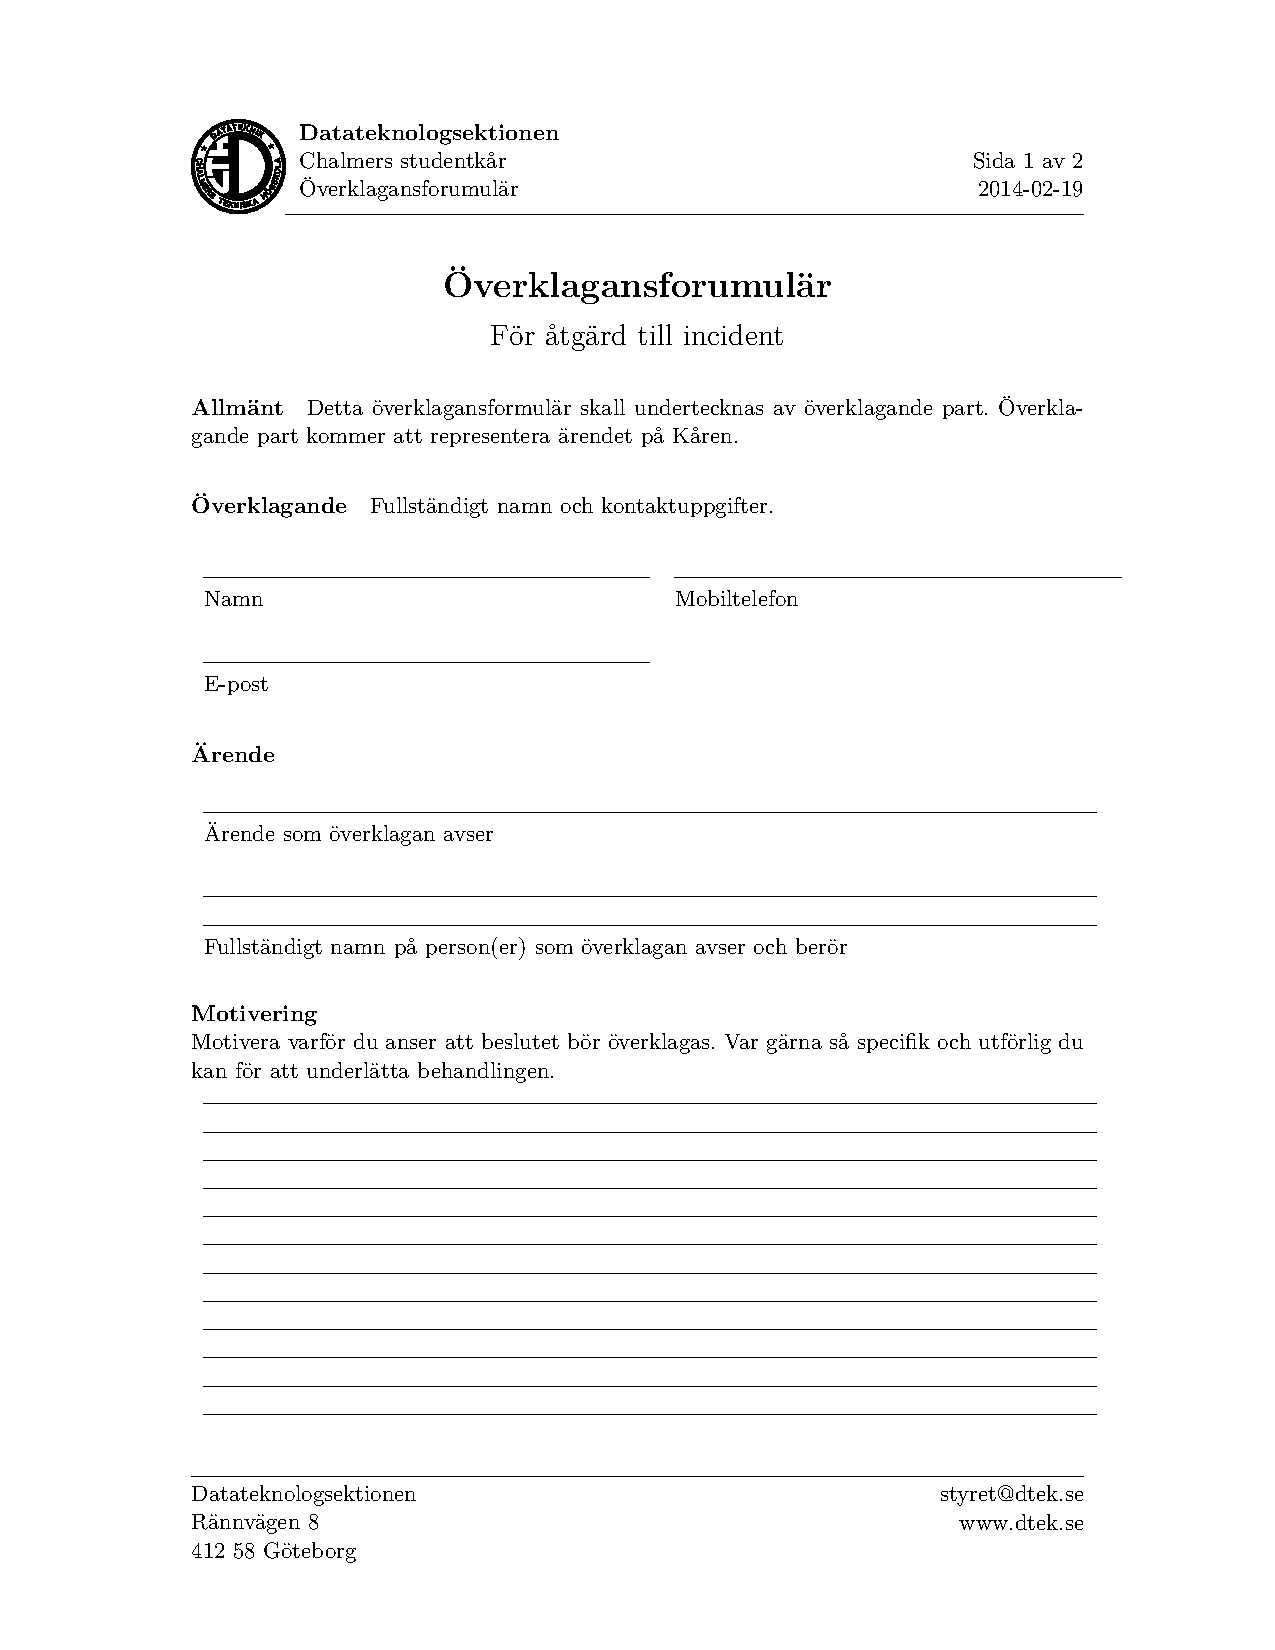
\includepdf[pages=-]{overklagan.pdf}

\end{document}
